%%%%%%%%%%%%%%%%%%%%%%%%%%%%%%%%%%%%%%%%%%%%%%%%%%%%%%%%%%%%%%%%%%%%%%%%%%%%%%%%
%2345678901234567890123456789012345678901234567890123456789012345678901234567890
%        1         2         3         4         5         6         7         8
% THESIS CHAPTER

\chapter{Usage Scenario}

\section{Scenario 1 [Marie Boucher]}
The Marie Boucher network \cite{dufournaud2017analyse}...
Summarise Marie Boucher background - I don't have this yet]

\begin{center}
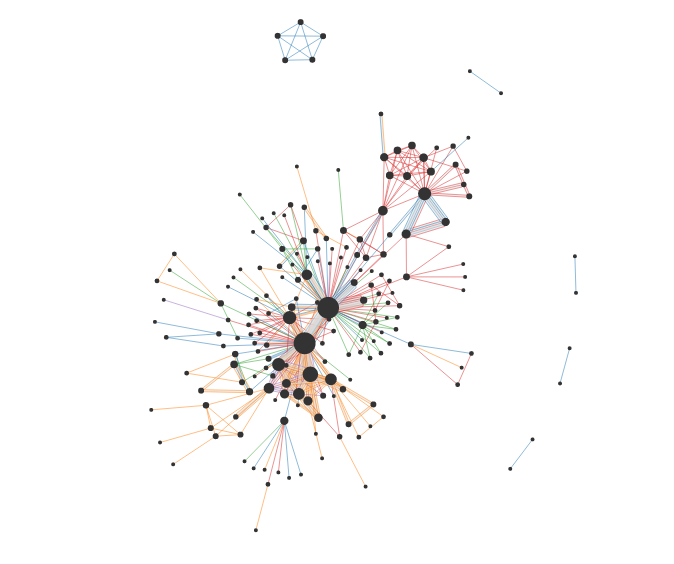
\includegraphics[trim={0 0 0 0}, width=140mm]{./Figures/marieBoucherFull.png}
\end{center}

-Only really one large component

-Some very central nodes

-Five satellite components

\begin{center}
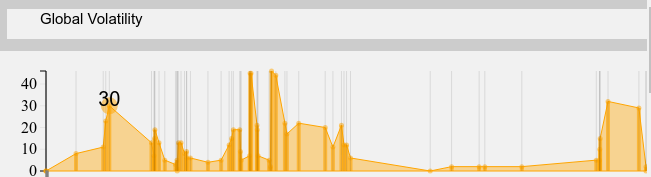
\includegraphics[trim={0 0 0 0}, width=140mm]{./Figures/marieBoucherGlobalVolatility.png}
\end{center}
I'll begin by looking only at the global measures, starting with global volatility we can see the network is initially erratic, then goes through very few changes for a sizeable portion of time, then has a burst of activity towards the end of the full period. 

\begin{center}
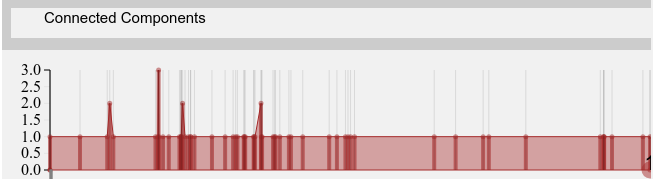
\includegraphics[trim={0 0 0 0}, width=140mm]{./Figures/marieBoucherConnectedComponents.png}
\end{center}
Looking next at the number of connected components we find that for the majority of time frames there is only one connected component - there are three frames with two connected components and one frame with three connected components. Manually stepping through the graph we can also see that these components tend to be connected to one of two highly central nodes.

\begin{center}
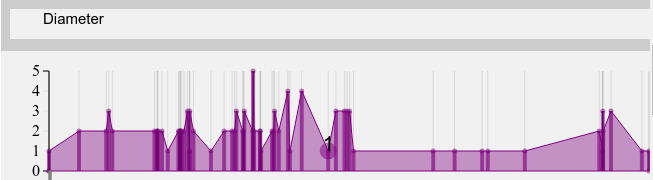
\includegraphics[trim={0 0 0 0}, width=140mm]{./Figures/marieBoucherDiameter.png}
\end{center}
Looking next at Diameter we see the same pattern we noticed in Global Volatility, erratic at first, a flat period of low activity then a jump at the end. There is a lot of variation in the values which could indicate that the network is quite different at each time frame. This is further enforced by density since it is similarly high in variation.

\begin{center}
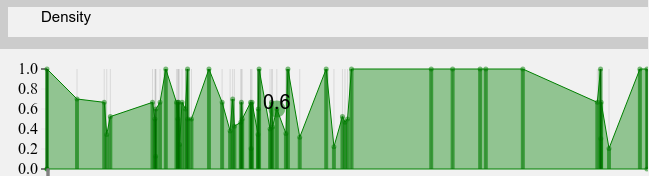
\includegraphics[trim={0 0 0 0}, width=140mm]{./Figures/marieBoucherDensity.png}
\end{center}

Density follows the same pattern. Interestingly the density during the flat period is 100\%. Investigating this with the timeline slider we see that this is because there are only ever two nodes connected at a time during this period. 
\begin{center}
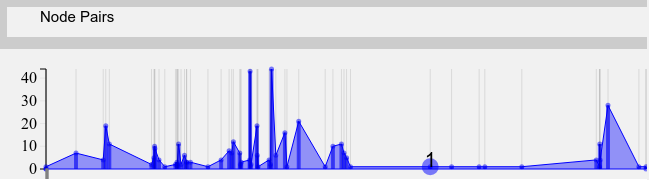
\includegraphics[trim={0 0 0 0}, width=140mm]{./Figures/marieBoucherNodePairs.png}
\end{center}
\begin{center}
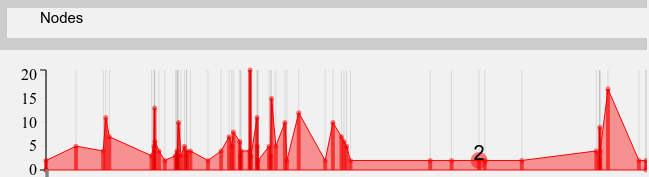
\includegraphics[trim={0 0 0 0}, width=140mm]{./Figures/marieBoucherNodes.png}
\end{center}
We could equally have confirmed this by looking at the number of node pairs and number of nodes - number of nodes is always 2 and number of nodepairs is always 1 during this flat period. The number of node pairs is very tightly correlated to the number of nodes here, the peaks could be worth further investigation as they are clearly periods of high activity relative to other frames.

\begin{center}
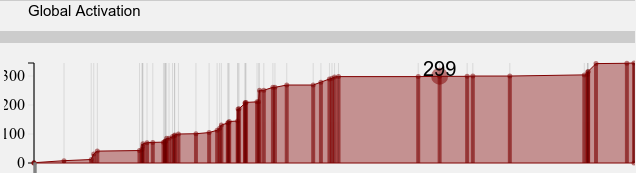
\includegraphics[trim={0 0 0 0}, width=140mm]{./Figures/marieBoucherGlobalActivation.png}
\end{center}
Global activation increases reasonably linearly for the first period. Notably during the flatter period it does increase slightly at each step confirming that the pairs we investigated in the density section are all different. 

\begin{center}
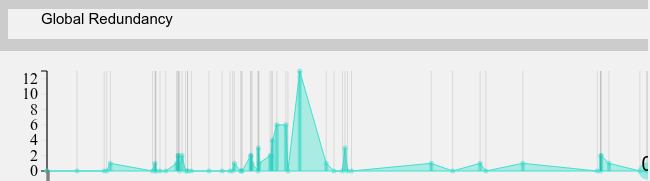
\includegraphics[trim={0 0 0 0}, width=140mm]{./Figures/marieBoucherGlobalRedundancy.png}
\end{center}
Global redundancy is mostly fairly low, however there is one large peak which indicates further investigation could be useful as to why only that frame had many previously seen nodepairs, particularly as that specific frame wasn't identified as interesting by any of the other measures. The burst of activity at the end we noticed earlier isn't as obvious in this graph, indicating that most of the connections made in that period are new.
    
Looking more generally at the graphs, the spacing of the vertical lines also indicates three separate periods. We can also spot some periods and frames where many graphs have notable peaks or troughs that could spark further investigation.
    
\begin{center}
\begin{tabular}{cc}
\label{marieBoucherLocalVolatilityFull}
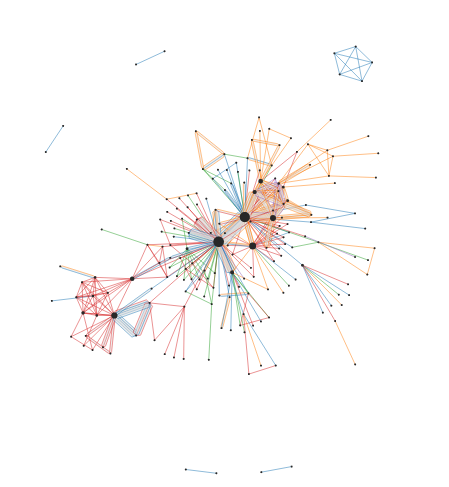
\includegraphics[trim={0 0 0 0}, width=140mm]{./Figures/marieBoucherLocalVolatilityFull.png}
\end{tabular}
\captionof{figure}{Marie Boucher - Local Volatility for a short period}
\end{center}   
Next, the local measures can be investigated. Applying local volatility to the whole graph, we see that the two highly central nodes have high volatilities. This is because they make many fresh connections. Other fairly central nodes can be seen to have noticeably high volatilites. Standout nodes of interest here are more obvious than when the centrality measure is applied.
\begin{center}
\begin{tabular}{cc}
\label{marieBoucherLocalCentralityFull}
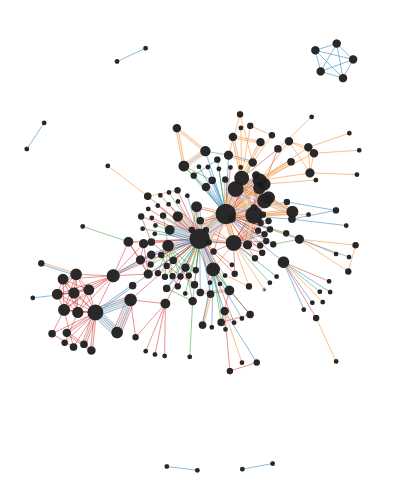
\includegraphics[trim={0 0 0 0}, width=85mm]{./Figures/marieBoucherLocalCentralityFull.png}
\end{tabular}
\captionof{figure}{Marie Boucher - Local Degree Centrality for the full period}
\end{center}   


\begin{center}
\begin{tabular}{cc}
\label{marieBoucherLocalRedundancyPeriod1}
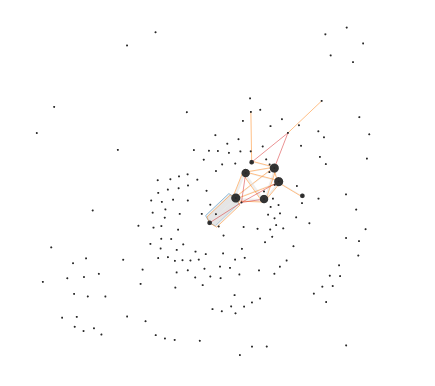
\includegraphics[trim={0 0 0 0}, width=85mm]{./Figures/marieBoucherLocalRedundancyPeriod1.png}
\end{tabular}
\captionof{figure}{Marie Boucher - Local Redundancy for a short period}
\end{center}   
Applying local redundancy to the network and stepping through it, there are few nodes that particularly stand out as having high redundancy, as expected the central nodes tend to have higher values than the outer nodes but some of the tightly linked nodes have notable redundancies, showing that they are connected a few separate times in the full period.

\begin{center}
\begin{tabular}{cc}
\label{marieBoucherLocalActivationPeriod1}
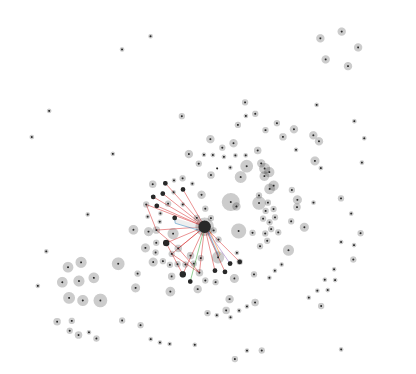
\includegraphics[trim={0 0 0 0}, width=140mm]{./Figures/marieBoucherLocalActivationPeriod1.png}
\end{tabular}
\captionof{figure}{Marie Boucher - Local Activation for a short period}
\end{center} 
Switching to activation and we can see many nodes score quite high as we step through the network. The central nodes in particular but also some of the outer nodes.

\section{Scenario 2 Turin Network}

[Reference and Summary]

The Turin network is much more seperated than Marie Boucher and much more cluster/component based. This makes it an excellent network to analyse alongside Marie Boucher.

\begin{center}
\begin{tabular}{cc}
\label{edgeTypes}
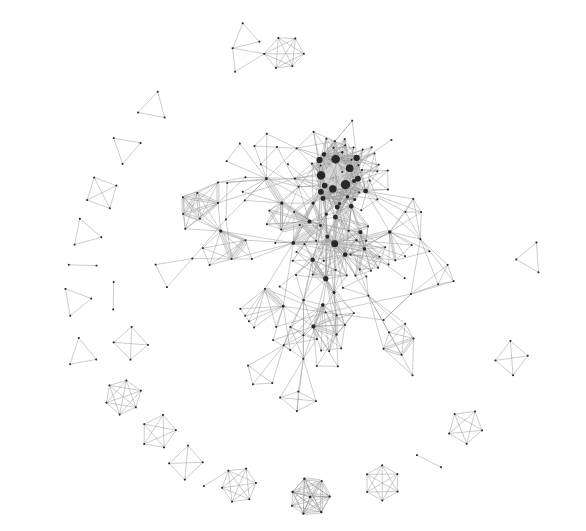
\includegraphics[trim={0 0 0 0}, width=140mm]{./Figures/TurinLocalVolatilityFull.png}
\end{tabular}
\captionof{figure}{The Turin Network, Local Volatility Measure Enabled}
\end{center}

We begin again by looking at the global measures. Global volatility has around five periodic large jumps.
\begin{center}
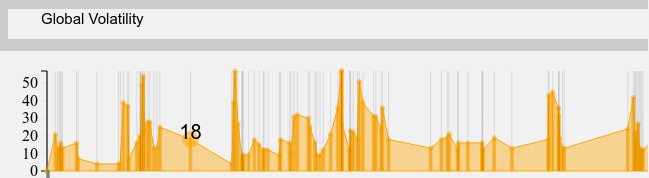
\includegraphics[trim={0 0 0 0}, width=140mm]{./Figures/TurinGlobalVolatility.png}
\end{center}   

In between each of these jumps is reasonably high volatility, so together these indicate that there are occasional very large changes in the network and that in general the network is quite volatile and never really static for a period of time.
    
\begin{center}
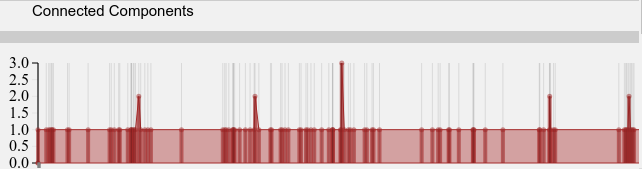
\includegraphics[trim={0 0 0 0}, width=140mm]{./Figures/TurinConnectedComponents.png}
\end{center}  
Looking next at the number of connected components - if we observe the network itself and step through it then it is readily apparent that it is made of many small connected components which tend to become active for short periods. Interestingly, what this graph shows - combined with this observation about the network, is that for the majority of the time there is only one active connected component, with only four time frames occurring with two active and one time frame occurring with three active.

\begin{center}
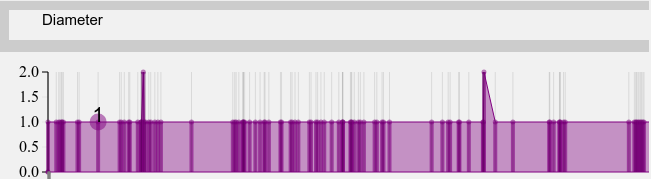
\includegraphics[trim={0 0 0 0}, width=140mm]{./Figures/TurinDiameter.png}
\end{center}
Diameter is equally interesting, there are only two time frames where the diameter is over one, and in both cases that value is two. Combined with what we know about connected components we can see that all of these components are highly connected since the vast majority only have a diameter of one, which is the smallest possible diameter for any network.
    
\begin{center}
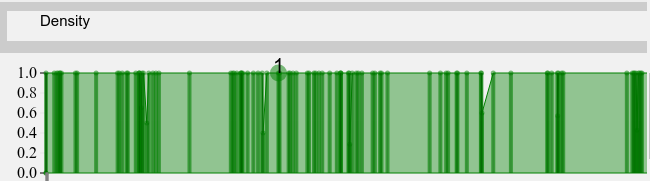
\includegraphics[trim={0 0 0 0}, width=140mm]{./Figures/TurinDensity.png}
\end{center}    
Adding density further consolidates these findings as we can see that for the majority of time frames the components have a density of 100\%. Combining this with what we've already discovered we now know that in most time frames we have a single connected component with every node in that component connected to every other node in that component. Two of the dips also align with the spikes in diameter.

\begin{center}
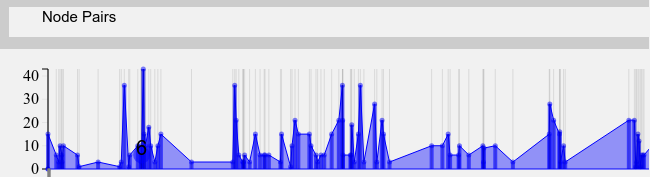
\includegraphics[trim={0 0 0 0}, width=140mm]{./Figures/TurinNodePairs.png}
\end{center}    
\begin{center}
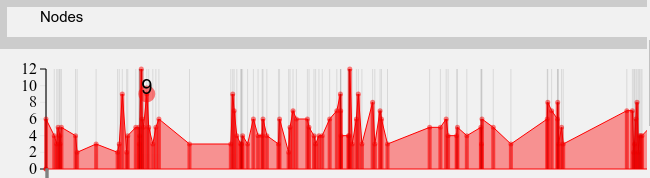
\includegraphics[trim={0 0 0 0}, width=140mm]{./Figures/TurinNodes.png}
\end{center}    
Due to the density and what we've observed previously, the number of nodepairs and nodes are naturally very tightly correlated. Comparing with the density graph we can see that the few blips in perfect correlation all match the fluctuations in density. Since we know this network tends to have one active fully connected component active in each time frame, we can now gain a sense of the sizes of each of these components. Comparing again with the connected components graph we can see that these large jumps tend to be linked with time frames where there is more than one connected component. Some of the blips in diameter and density also align with time frames with more than one connected component. The time frames these blips occur in could therefore be worth extra investigation.
    
\begin{center}
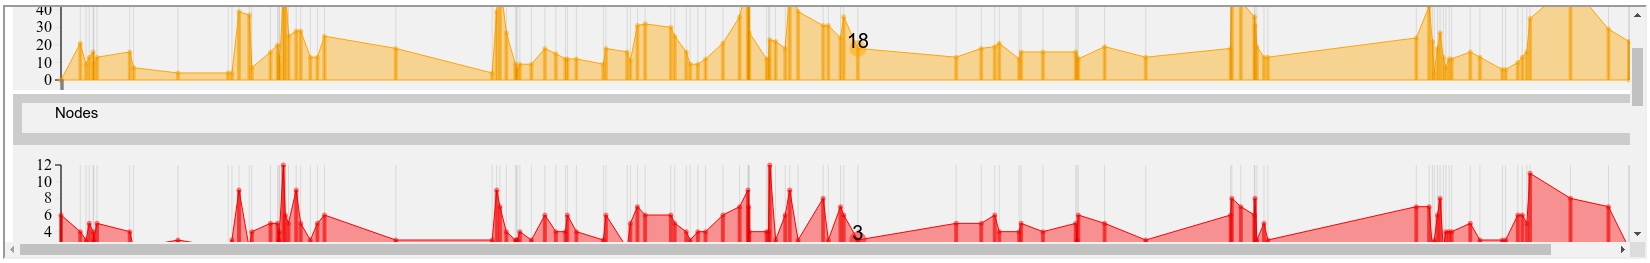
\includegraphics[trim={0 0 0 0}, width=140mm]{./Figures/TurinGlobalVolatilityAndNodes.png}
\end{center}        

Comparing number of nodes with Global Volatility by dragging the number of nodes graph up such that it is directly below the global volatility graph they can now be easily compared. We can see that the steps of very high volatility identified earlier are explained by the large new connected components appearing during those time frames.
   
\begin{center}
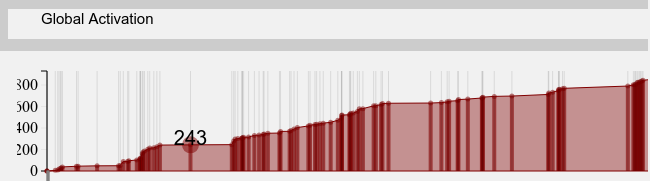
\includegraphics[trim={0 0 0 0}, width=140mm]{./Figures/TurinGlobalActivation.png}
\end{center}       
Continuing down to Global Activation we can see that new nodepairs are added at a fairly constant pace. Looking next at Global Redundancy, the peaks indicate that many of the nodepairs have been active before, we can use this alongside the network itself to easily find the components that appear more than once.
    
\begin{center}
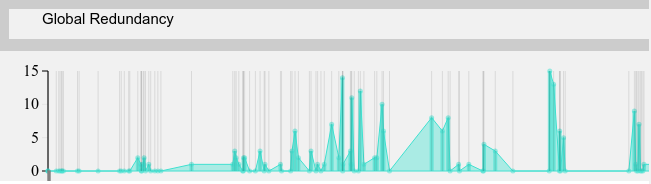
\includegraphics[trim={0 0 0 0}, width=140mm]{./Figures/TurinGlobalRedundancy.png}
\end{center}
Finally with Global Redundancy, the values appear highly erratic. This measure would be useful to see at which periods past business groups are reconnected. Dragging it to compare it with Global Volatility and Nodepairs we can see some correlation.


Looking more generally at all graphs we can gain some more insight. Looking at the spread of time frames by observing the vertical bars, we can identify periods of no change and periods of considerable change. 
    
\begin{center}
\end{center}

\begin{center}
\begin{tabular}{cc}
\label{edgeTypes}
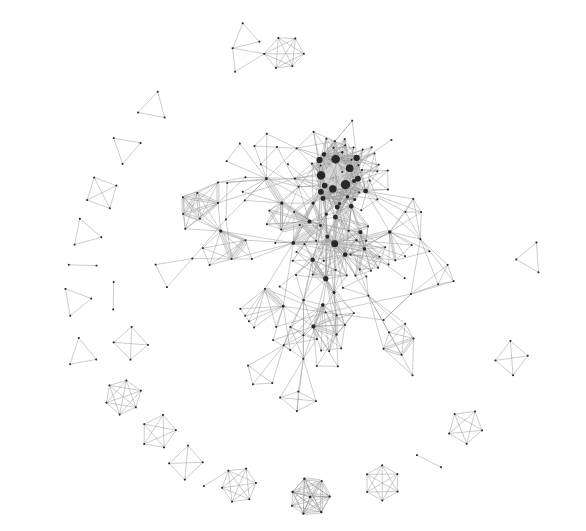
\includegraphics[trim={0 0 0 0}, width=140mm]{./Figures/TurinLocalVolatilityFull.png}
\end{tabular}
\captionof{figure}{Turin Local Volatility - Full time period}
\end{center}
Next, we can experiment with the local measures. First with volatility, stepping through the network with a minimal window we see that the connected components tend to all have low similar volatilities with no standout nodes. Observing the full network over the whole time period we see that there is a large cluster containing several highly volatile nodes. Stepping through the graph we see that this is because many of the connected components overlap in some way within this cluster of nodes. These nodes are therefore very worthy of further investigation as they are highly active and with many different nodes rather than a fixed number.


\begin{center}
\begin{tabular}{cc}
\label{edgeTypes}
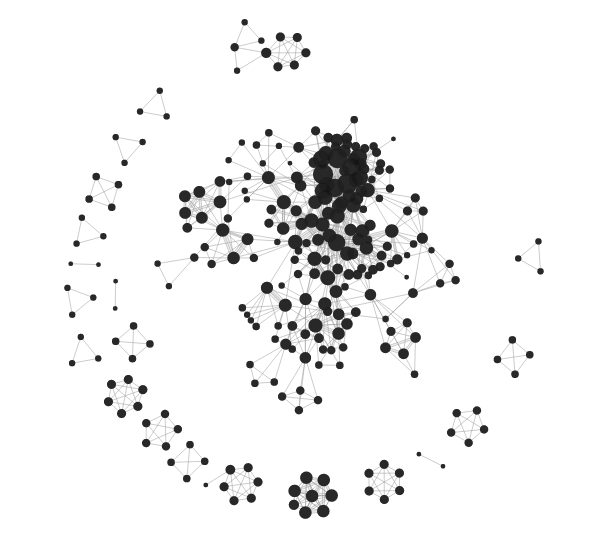
\includegraphics[trim={0 0 0 0}, width=140mm]{./Figures/TurinLocalCentralityFull.png}
\end{tabular}
\captionof{figure}{Turin Centrality - Full time period}
\end{center}

\begin{center}
\end{center}
Comparing these results from local volatility with the centrality measure - again applied to the whole graph - is interesting, because we can see that using local volatility makes the interesting nodes stand out much more. 
\begin{center}
\begin{tabular}{cc}
\label{edgeTypes}
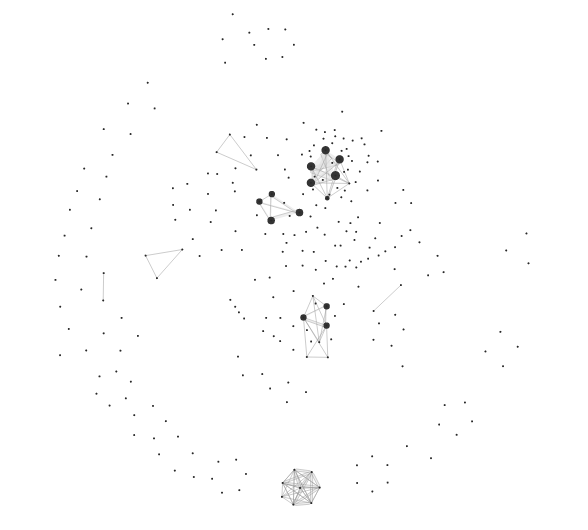
\includegraphics[trim={0 0 0 0}, width=140mm]{./Figures/TurinLocalRedundancy1.png}
\end{tabular}
\captionof{figure}{Turin Local Redundancy - short time period}
\end{center}
Switching to local redundancy and selecting a period towards the end of the network's timeline we can easily spot the components that have been active at some point before that period as they have a redundancy $> 0$.


\begin{center}
\begin{tabular}{cc}
\label{edgeTypes}
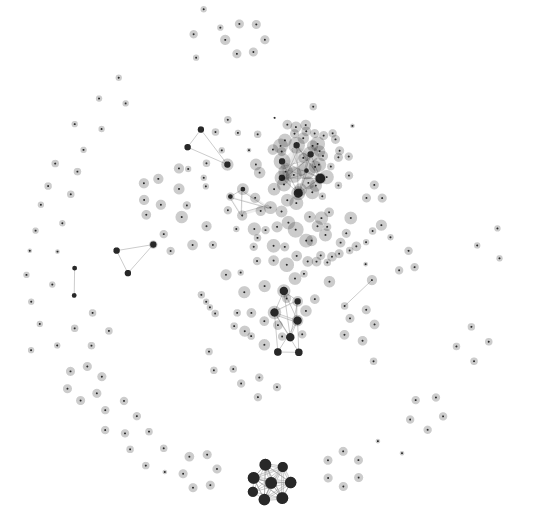
\includegraphics[trim={0 0 0 0}, width=140mm]{./Figures/TurinLocalActivation.png}
\end{tabular}
\captionof{figure}{Turin Local Activation - same short time period}
\end{center}
This further complements our findings from the global redundancy measure. Switching directly to local activation from here and looking again at the components identified as having higher redundancy we can see how high the activation in the selected time period is relative to the total network activity by comparing with the grey outer circles. Since they aren't considerably larger for any node in these components we could infer that this component is likely only fully active one or two times before this period.

\section{Scenario 3 - Marguerite} 

\begin{multicols}{2}
\begin{center}
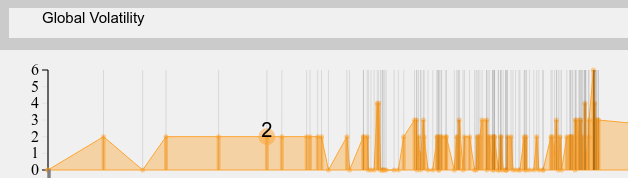
\includegraphics[trim={0 0 0 0}, width=70mm]{./Figures/margueriteGlobalVolatility.png}
\end{center}
\begin{center}
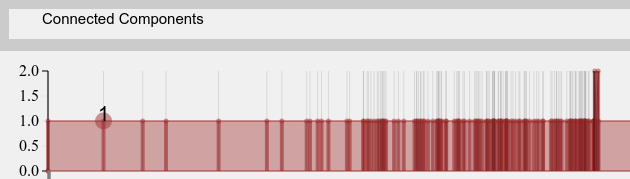
\includegraphics[trim={0 0 0 0}, width=70mm]{./Figures/margueriteConnectedComponents.png}
\end{center}
\begin{center}
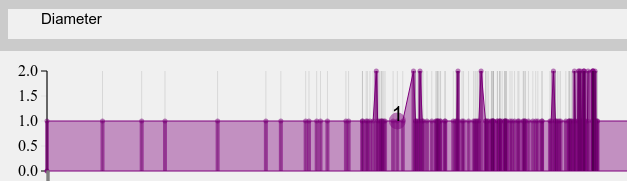
\includegraphics[trim={0 0 0 0}, width=70mm]{./Figures/margueriteDiameter.png}
\end{center}
\begin{center}
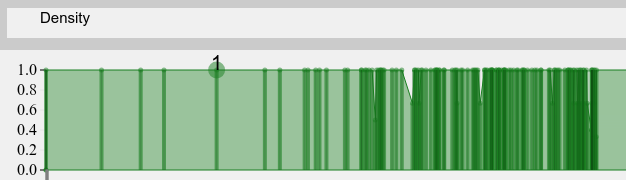
\includegraphics[trim={0 0 0 0}, width=70mm]{./Figures/margueriteDensity.png}
\end{center}
\begin{center}
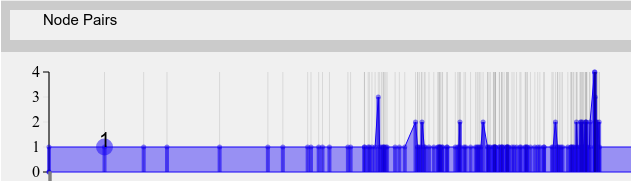
\includegraphics[trim={0 0 0 0}, width=70mm]{./Figures/margueriteNodePairs.png}
\end{center}
\begin{center}
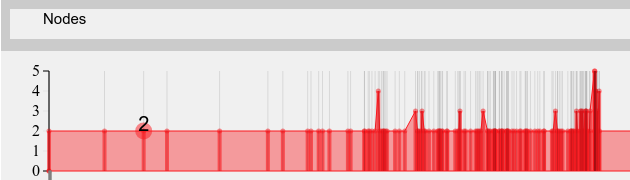
\includegraphics[trim={0 0 0 0}, width=70mm]{./Figures/margueriteNodes.png}
\end{center}
\begin{center}
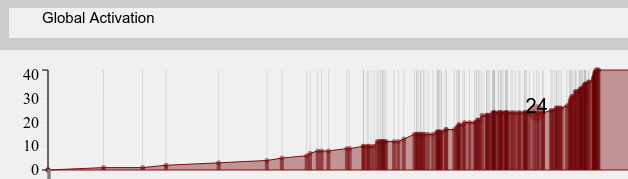
\includegraphics[trim={0 0 0 0}, width=70mm]{./Figures/margueriteGlobalActivation.png}
\end{center}
\begin{center}
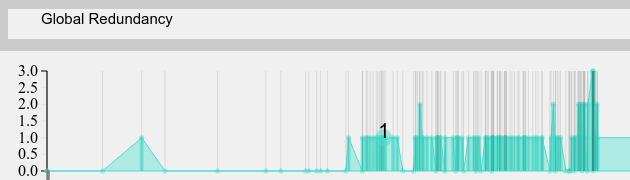
\includegraphics[trim={0 0 0 0}, width=70mm]{./Figures/margueriteGlobalRedundancy.png}
\end{center}
\columnbreak
[Reference]
Finally, to assess the power of the measure based approach, we could try looking solely at the global measures of a new network to see how much information we can gleam. 

Looking generally at all graphs we can see there is fairly little activity in the first half and then a lot in the second. We can see that for most time frames there are only two nodes involved - explaining the density and diameter - and steadily increasing global activation implying that many new nodes are connected to. What's very interesting however is that global redundancy for the second half tends to be one. Tying this together and the picture we get is either of a network primarily composed of one node connecting to many new nodes in the second period or many pairs becoming active where one of the nodes in the pair has been active before. Looking more closely at the values of global activation which appear to increase by one during each time frame in this period and we can rule out the second option.
\end{multicols}

Looking at the actual network, these findings were accurate. 
\begin{center}
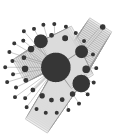
\includegraphics[trim={0 0 0 0}, width=40mm]{./Figures/margueriteNetwork.png}
\end{center}
[Summary and reference for the Marguerite network.]
Of course, the measures are meant to be complementary to the network and not to replace it, but being able to extract this much information solely from them with relative ease indicates that they are a powerful tool.



\chapter{Conclusion}

\section{Potential further work} 
Creating visualisations is a highly iterative and experimental process, so naturally many ideas have been produced for improvements that could be made. 
One of the most immediately useful would be implementing automatic point of interest detection. Specific frames of the network where most measures changed noticeably compared with previous values would be highlighted on the timeline.
\newline

Another improvement mentioned during the feedback meeting (and briefly considered before) was enabling graphs to be exported as a png to allow for easy insertion into academic papers. This would encourage adoption and improve quality of life for end users.
\newline

Adding the ability to move the databar into a separate window, which could then be dragged to a separate screen - creating more space for the node-link diagram and allowing more graphs in the databar to be visualised at once. 
\newline

Running a think-aloud study or similar user trial could be useful to discover more about how effective the current implementation is and provide insight into further improvements.
\newline

Adding more measures is an obvious improvement - particularly local dynamic measures as they aren't found in other tools. An example could be a measure to add a sense of node 'promiscuity' - if volatility focuses on how the lifespans of node-pairs vary over time then 'promiscuity' would focus more on how often those edges tend to be with the same nodes. A node that had a few fairly rigid connections but also made a new connection every time step would have relatively low volatility but high promiscuity. A node that erratically gained and lost connections but only to a select few nodes would have high volatility but low promiscuity.

Could add selecting/locking a time period instead of using the entire period for the greyed out backing circles for the nodes

\section{Evaluation of work completed} 
The system works well in the described usage scenarios. The complementary approach taken means that...
